\section{Method}

As a consequence of the errors described in the previous section, there is such a variance in the sequences that we can not expect to see a true allele in any one of the reads of an individual. A first step to attack this problem is to make an alignment of all the sequences of a individual in such a way that each nucleotide end up in its correct position of the 270 base pair long sequence. This implies that we need to identify where in the sequences there is missing data, that is a machine induced deletion, and where the machine have made false insertions. A satisfying result could look like in figure \ref{fig:dream_scenario}

\begin{figure}[ht]
	\centering
		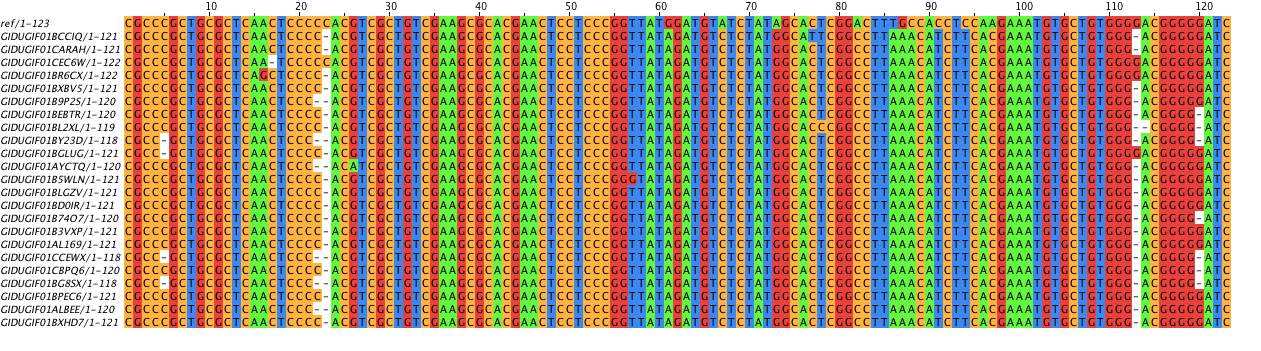
\includegraphics[width=\textwidth]{../pictures/align_with_ref_cropped.png}
	\caption{Aligned sequences. Picture does not show the full sequence.}
	\label{fig:dream_scenario}
\end{figure}


When the alignment is done we need to figure out what parts of the sequences that holds information about the true alleles and what parts that are chimeric formations or machine errors. The problem can be divided into two main parts with two separate methods to handle them. We start this section with an overview of the workflow, the steps are described in more detail in the following section:

\begin{enumerate}
	\item Align the reads
	\item Identify the alleles
\end{enumerate}

\subsection{Process Overview}

\begin{itemize}
	\item \textbf{Alignment} \\
	
	\textbf{Data in:} One file in fasta format for each of the individuals with raw sequence data.\\
	\textbf{Data out:} One file in fasta format for each of the individuals aligned sequences.\\
	
	% Indata Utdata
	
	\begin{enumerate}
		\item \textbf{Add tags}.\\ 
		\textbf{for each} reference sequence:\\
		Add the same tags that were used for sequencing, these are present in all of our data but not in the references.
		\item \textbf{Build reference }.\\% Varför dynamisk, kanske ska heta profile (PSSM)
		\textbf{for all} reference sequence:\\
		Look at the frequency of \emph{A,C,G,T} in every position to estimate the scores for each bases in each position.
		The result is a unique scoring scheme for each position that we call a Reference Profile.
		\item \textbf{Align the sequences}.\\
		\textbf{for each} sequence in each individual:\\
		Align the sequences globally, pairwise with the most abundant reference sequence (known as 00101) using the reference profile.
	\end{enumerate}
	\item \textbf{Choose Alleles} \\ 
	
	\textbf{Data in:} One file in fasta format for each of the individuals with aligned sequences.\\
	\textbf{Data out:} A fasta formatted file with one or two alleles for each individual.\\
	
	\begin{enumerate}
		\item \textbf{Find the variable positions}.\\
		\textbf{for each} individual:\\
		Find out what are true differences and what is errors among the reads of an individual.
		\item \textbf{Start building the alleles}.\\
		\textbf{for each} individual:\\
		Walk trough each position in the sequence and add it to the two alleles. If there is a variation in a position, find out which variation belongs to which allele and add them to the correct one. 
		\item \textbf{Compare with reference}.\\
		\textbf{for each} allele:\\
		Compare the alleles to all reference sequences pairwise to see which of the references that is most similar to the group.
		\item \textbf{Complete the alleles}.\\
		\textbf{for each} allele in each individual:\\
		Fill the deleted bases with the corresponding base from the most similar reference sequence.
		\item \textbf{Remove tags}\\
		\textbf{for each} sequence in each individual:\\
		Remove the tags.
	\end{enumerate}	
\end{itemize}
